% !TeX root = ./T15_report.tex

\section{Experiment 2}

\subsection{Theoretical Backround}

The goal of this experiment was to measure the cooling process of hot water in a Cup an predicting the end(room)-temperature. The temperature is expected to be described by the exponential curve
\begin{equation}
    T(t) = (T_0-T_R)e^{-kt}-T_R
\end{equation}

\noindent
where $T_0$ is the start temperature, $T_R$ room temperature and $1/k$ the time, when $T(t)-T_R$ has dropped by $\frac{1}{e}$.

\subsection{Execution}

\begin{figure}[H]
    \centering
    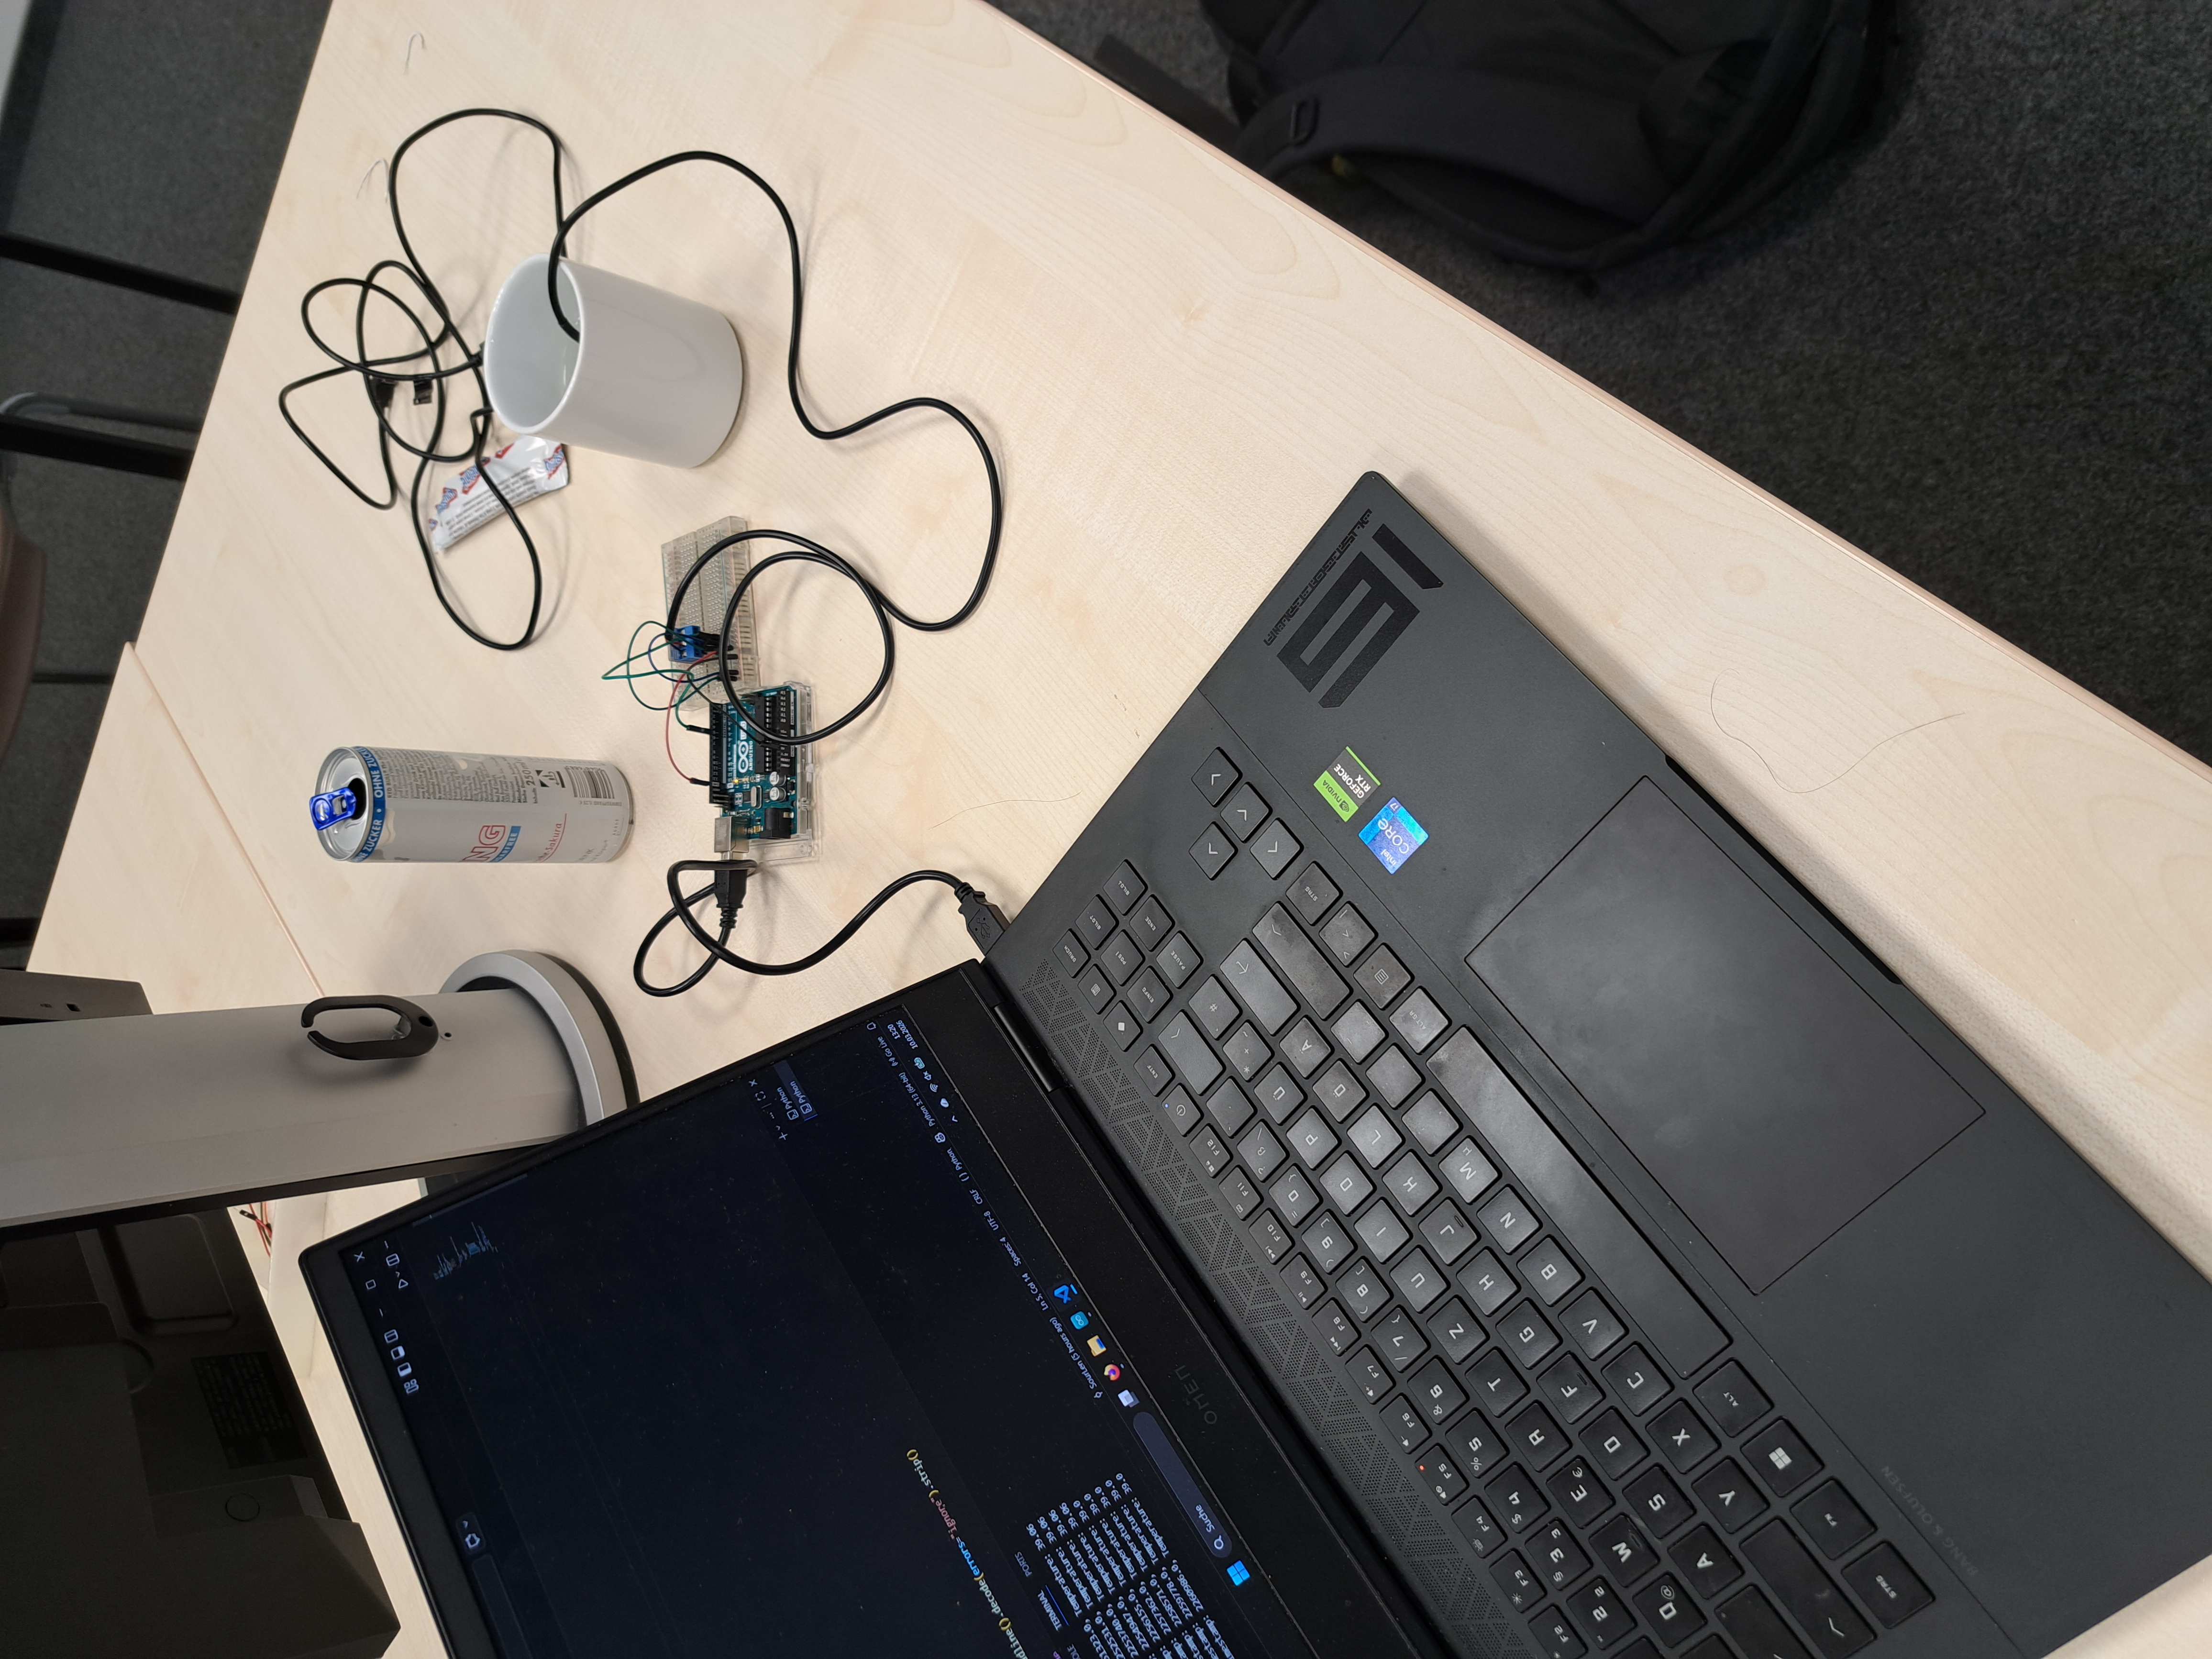
\includegraphics[height=5cm]{../temp_figures/exp2/exp2_1.jpg}
    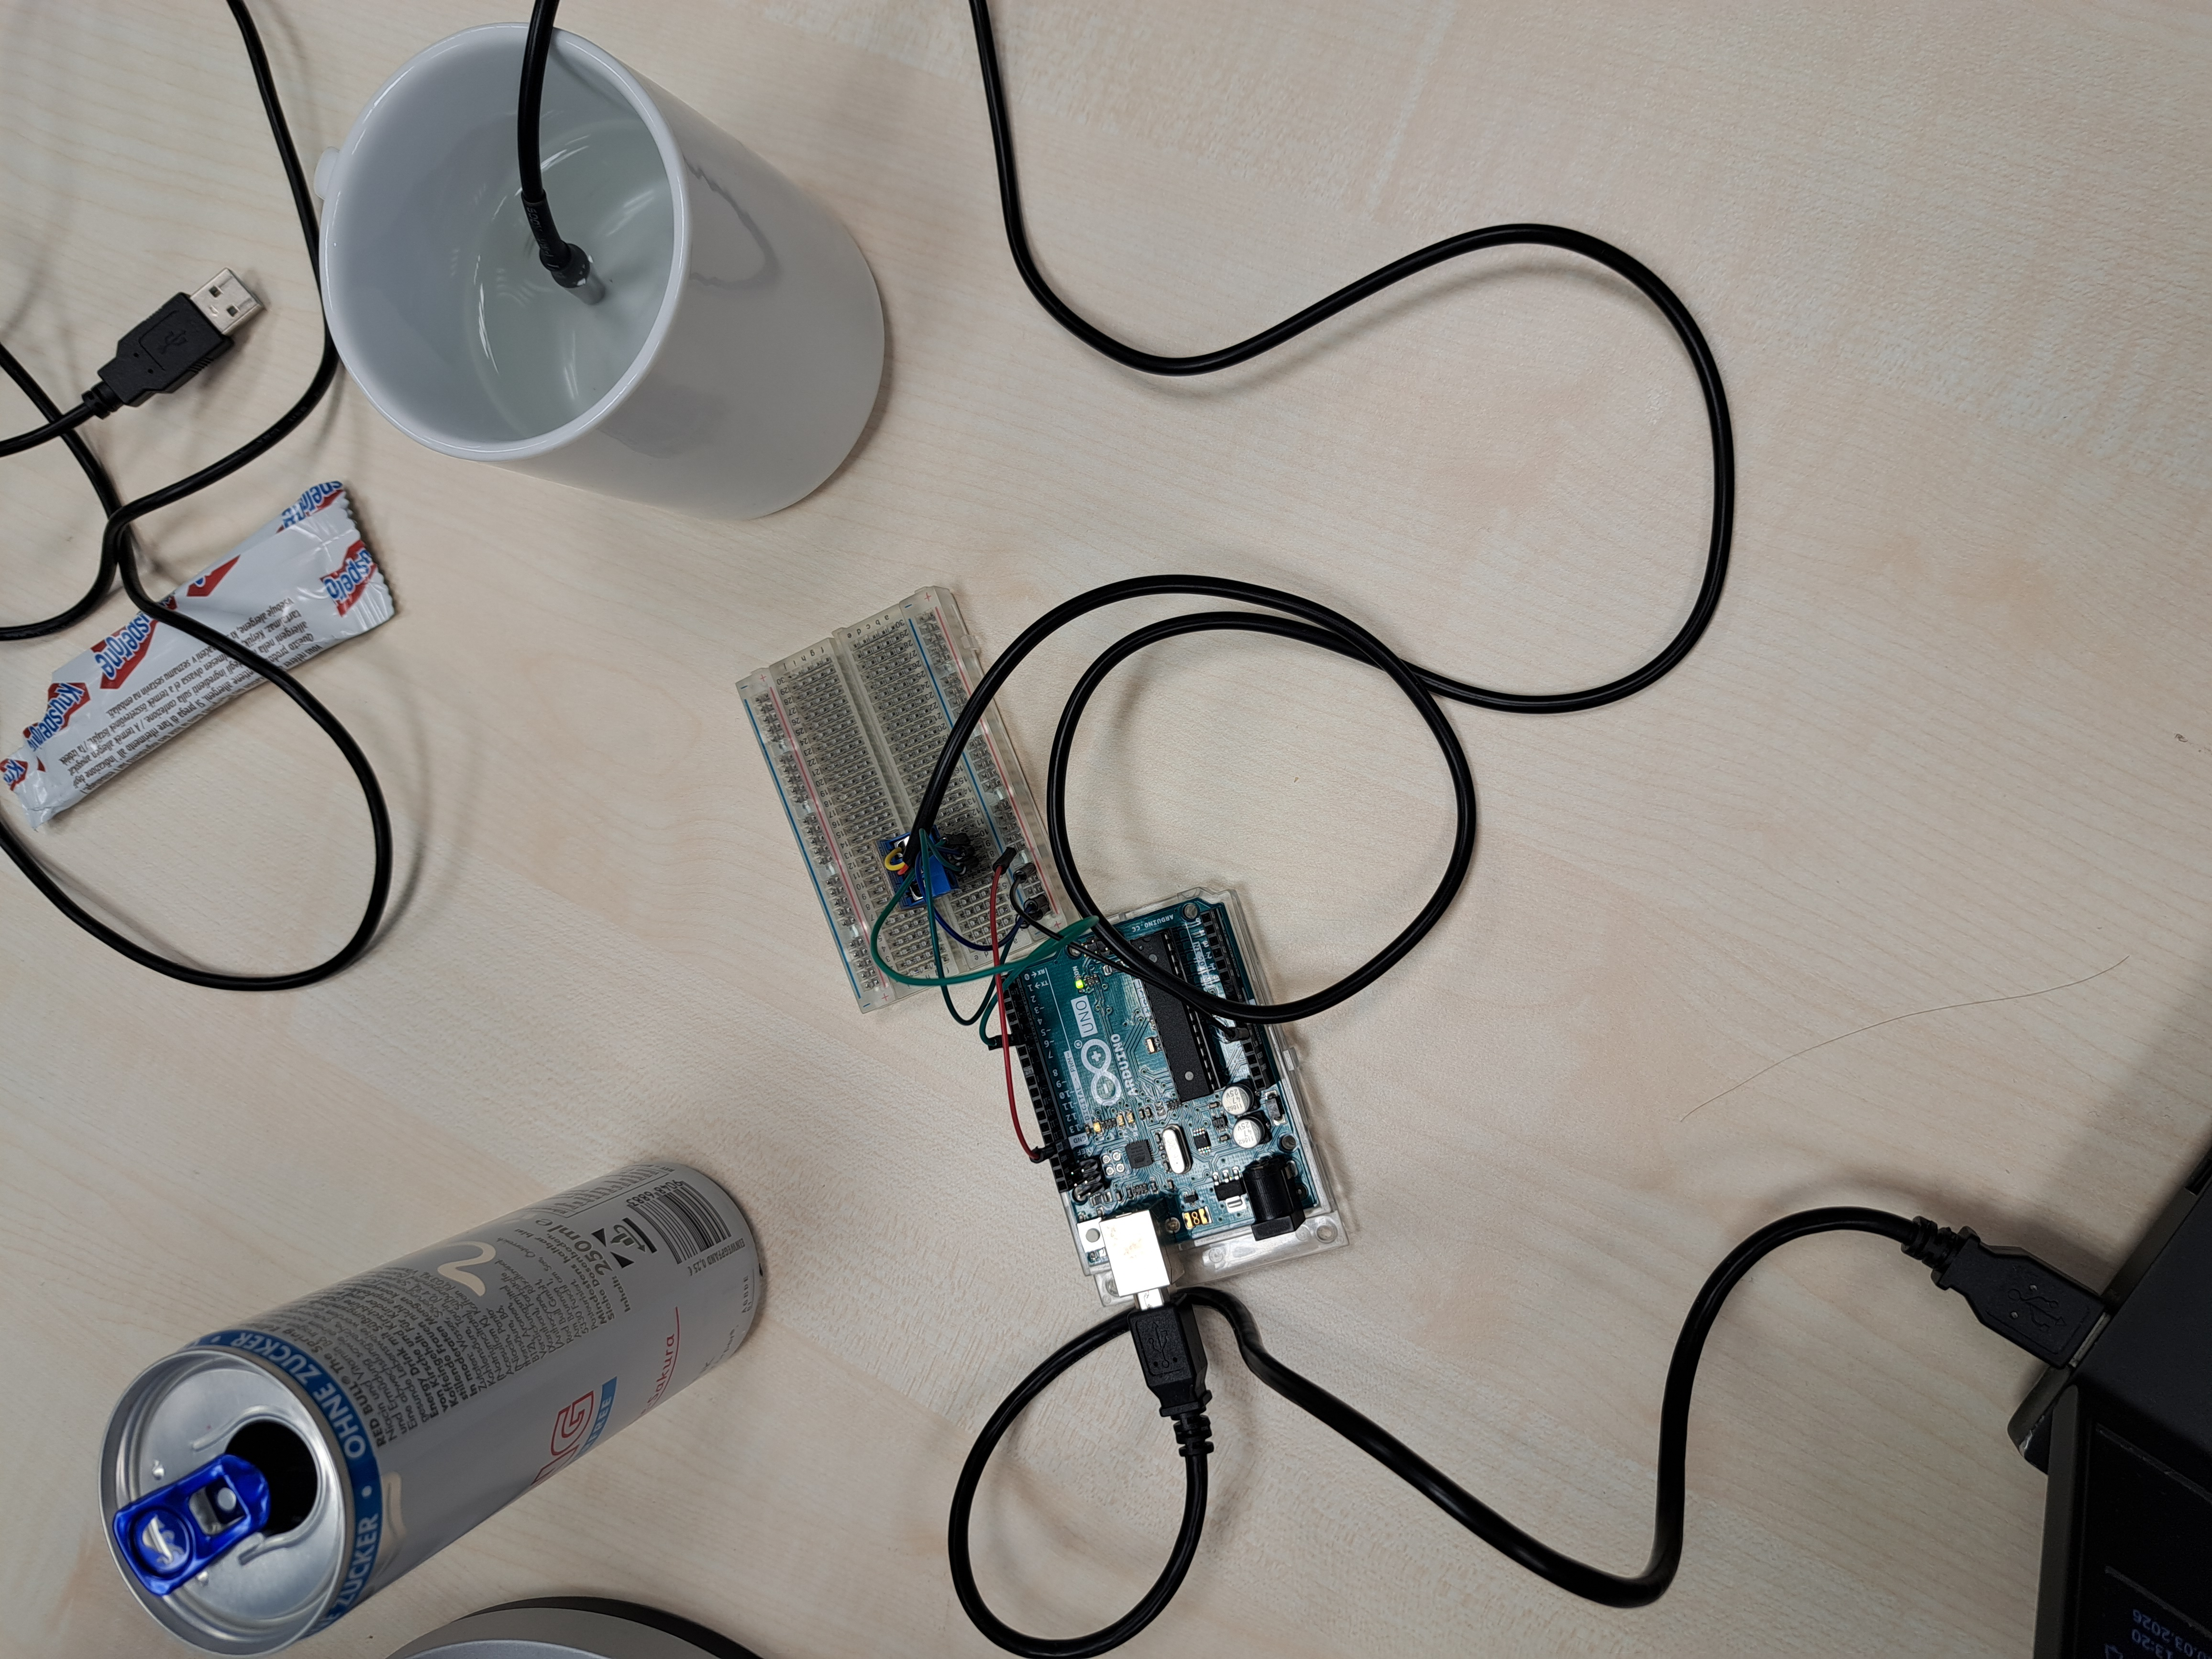
\includegraphics[height=5cm]{../temp_figures/exp2/exp2_2.jpg}
    \caption{Pictures of the set up}
    \label{exp2picture}
\end{figure}

As shown in \ref{exp2picture}, we used the setup as described in the instruction including the \textsf{S18B20 Waterproof Termperature sensor} and the \textsf{Arduino Uno}, again connected to our Laptop. Using a USB cable we adressed the Arduino implementing following code in the Arduino IDE

\inputminted[bgcolor=lightgray]{c}{../experiments/exp2/arduino/2_sketch.ino}

\noindent
Using this sketch the Arduino reads the sensor every 0.5 seconds and prints the temperature as well as the internal time.\\
To read and save the data we again used a python script on our laptop.

\inputminted[bgcolor=lightgray]{python}{../experiments/exp2/python/2.py}

\subsection{Results}

First, lets take a look at the error. The manufactorer \cite{data_DS18B20} states an accurracy of $\pm 0.5$. Dividing it by $\sqrt{3}$ gives us the uncertainty
\begin{equation}\label{man}
    \sigma_{\text{man}} = \frac{0.5}{\sqrt{3}}\unit{\celsius} \approx 0.29 \unit{\celsius}.
\end{equation}
Further we take a look at the digitalization error. 
\begin{figure}[H]
    \centering
    \label{last30}
    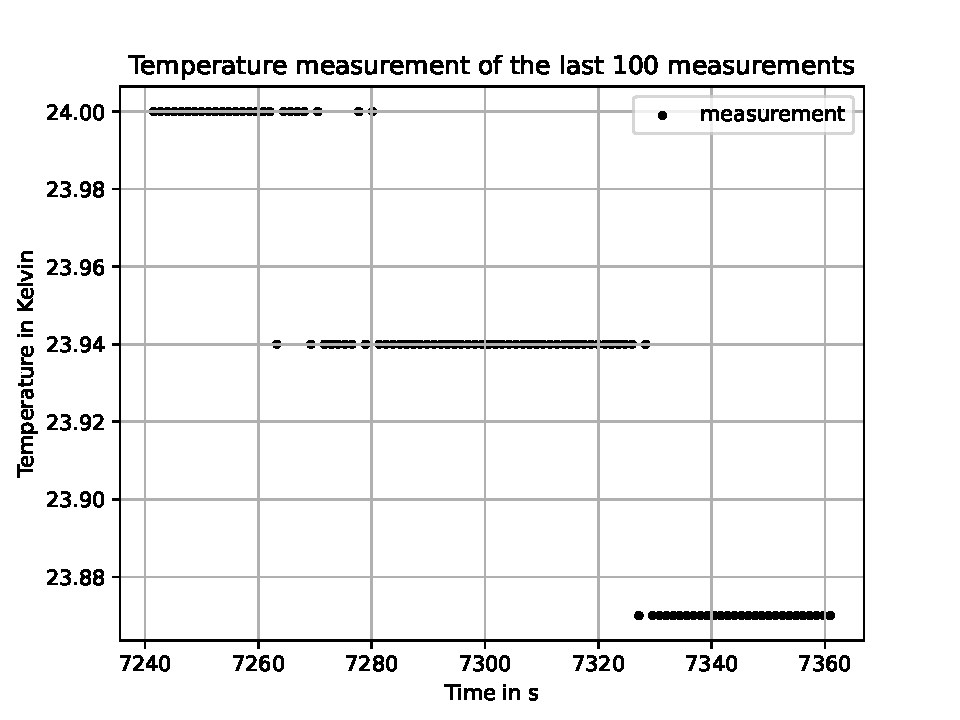
\includegraphics[width=0.8\textwidth]{../temp_figures/exp2/2_1.pdf}
    \caption{Plot of the last 30 measurements}
\end{figure}
\noindent
As we can see, the smallest step of the sensor is $0.065 \unit{\celsius}$. Dividing it by $\sqrt{12}$ grants us the digitalization uncertainty
\begin{equation}\label{dig}
    \sigma_\text{dig}=\frac{0.065}{\sqrt{12}}\unit{\celsius} \approx 0.02 \unit{\celsius}.
\end{equation}
Lastly we calculate the standart derviation of our noise measurement and recieve
\begin{equation}\label{noise}
    \sigma_\text{noise} \approx 0.03 \unit{\celsius}.
\end{equation}
Using \ref{man}, \ref{dig} and \ref{noise} we calculate the total uncertainty
\begin{equation}
    \sigma = \sqrt{\sigma_{\text{man}}^2 + \sigma_\text{dig}^2 + \sigma_\text{noise}^2} = 0.29 \unit{\celsius}.
\end{equation}

\noindent
Using this uncertainty we fit the theoretical curve to our measurement data and recieve
\begin{figure}[H]
    \centering
    \label{fit}
    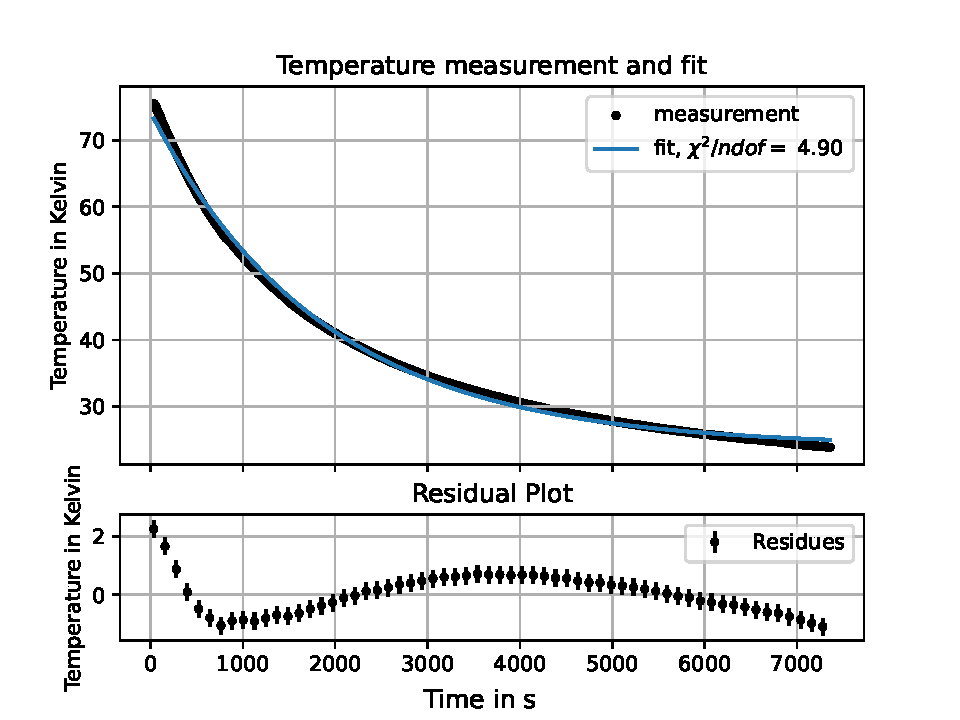
\includegraphics[width=0.8\textwidth]{../temp_figures/exp2/2_2.pdf}
    \caption{Plot of the fitted }
\end{figure}
\noindent
with the parameters
\begin{equation*}
    \begin{aligned}
        T_R &= (24.0138\pm 0.0005) \unit{\celsius}\\
        T_0 &= (74.214\pm 0.002)\unit{\celsius}\\
        k &=(5.359381463\cdot 10^{-4} \pm 0.000000009)\cdot 10^{-4} \unit{\second^{-1}}
    \end{aligned}
\end{equation*}
\noindent
The predicted Room temperature does fit the expected value. However, we have a $\chi^2=4.9$. Looking at the plot of the residues, the error seems to be of systematic natur. As a reason, we suspect that the cooling of the room temperature by opening the windows has an effect on the measurement.\\
A more fitting model considers this behavior by looking at the Time dependency of $T_R \to T_R(t)$. We expect this additional time dependency to be small so we only consider terms to the first order.
\begin{equation}
    T(t) = (T_0-T_R(1 + at))e^{-kt}-T_R(1 + at)
\end{equation}
\noindent
This new approach results in a more accurate describtion of the process at the cost of the meaningfulness of the fit parameters with
\begin{equation*}
    \begin{aligned}
        T_R &= (34.954\pm 0.001) \unit{\celsius}\\
        T_0 &= (76.25\pm 0.0003)\unit{\celsius}\\
        k &=(7.99040211 \pm 0.00000002)\cdot 10^{-4} \unit{\second^{-1}}\\
        a &=(-4.493482592 \pm 0.000000002)\cdot 10^{-5} \unit{\second^{-1}}
    \end{aligned}
\end{equation*}
\noindent
Apart from this issues, the new model delivers a way better description of the measurement.
\begin{figure}[H]
    \centering
    \label{fit_new}
    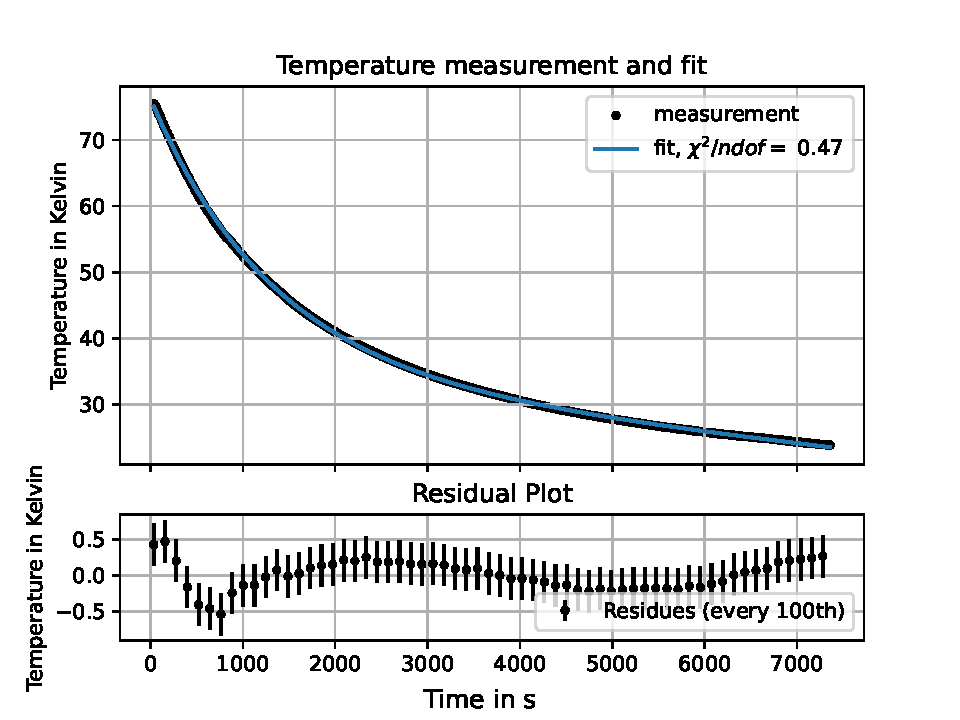
\includegraphics[width=0.8\textwidth]{../temp_figures/exp2/2_3.pdf}
    \caption{Plot of the new fitted model}
\end{figure}
\noindent
The new $\chi^2$ of $0.46$ is a good indicator for the model being more fitting, even though it being so low is a sign ob a slight overestimation of the real error on the data.\\
In comparison, the normal model does seem to deliver a good estimation of the parameters, though lacking in the description of the measurements while the addition of a linear term seemingly fixes that issue at the cost of the parameters meaning. The truth lies somewhere between those two ideas.